% -------------------------------------------------------------------------------------------------
%      MDSG Latex Framework
%      ============================================================================================
%      File:                  introduction-[UTF8,ISO8859-1].tex
%      Author(s):             Michael Duerr
%      Version:               1
%      Creation Date:         30. Mai 2010
%      Creation Date:         30. Mai 2010
%
%      Notes:                 - Example chapter
% -------------------------------------------------------------------------------------------------
%
\chapter{Related Work}\label{sec:RelatedWork}
% - Definition of field of research \\
% - Scientific Scope \\
% - Which comparable work in research exists? \\
% - Separation from other works
Realistic RL scenarios often involve multiple agents solving problems together, for example robots working in warehouses and factories. Such multiagent environments come with many difficulties. On one hand, in a scenario where agents work independently, it is very probable that they get in each other's way. They aim to achieve the highest score or finish their individual tasks, preventing the overall goal to be achieved.

In cooperative environments, on the other hand, agents share the reward and therefore can not tell who contributed useful actions. 
%Hence, all agents receive the same reward regardless of their contribution, which aggravates learning.
The difficulties of agents working independently is discussed in Chapter \ref{market} whereas the cooperation challenge is the focus point of the next Chapter.

\section{Credit Assignment Problem}\label{CAP}
Sutton and Barto \cite{suba18} define a RL environment as cooperative, when agents execute their actions collectively each time step but receive one overall reward in return. In this case, individual learning is difficult or even impossible. Collective actions may contain bad choices that would be rewarded or, in case of a penalty, good actions that would be punished. Deciding which agent deserves more or less of the common reward is referred to as the credit assignment problem (CAP) \cite{mi61}.

The CAP originated in a one-agent environment that only returned reward once the goal is reached or the terminating condition applied. A popular example of this is a chess game. In 1961, Minsky \cite{mi61} elaborated on this by explaining that a player wins or loses the game, but cannot retrace which decision got him there. Later on, Sutton decomposed the CAP into subproblems, namely the structural and temporal CAP \cite{su84}. He suggests, that the temporal problem lies in assigning credit to each chess move by determining when the position improves or worsens, rewarding or penalizing that certain action. On the contrary, the structural CAP is assigning credit to the internal decision that leads to each particular action.

% Sutton also refers to a chess game to explain the subproblems. 
Transferring the single-agent CAP into a multiagent environment, Agogino and Tumer \cite{agtu04} imply that the problem shifts from being of temporal to structural type. They explain that while a single agent faces the temporal CAP due to many steps taken within an extended time period, in the multiagent case it becomes a structural CAP because of multiple executed actions in a single-time-step. Since the actions are executed all at once, the challenge is now evaluating the decision that lies underneath.
% They explain that a single agent faces the temporal CAP when many steps are taken within an extended time period so learning from the returned reward at the end is problematic. Whereas in the multiagent setting it becomes a structural CAP because of multiple actions leading to a shared reward during a single-time-step.

Over the years many solutions and theories emerged in order to solve CAPs in multiagent environments \cite{rabe09}, \cite{zhli20}, \cite{agtu04}. A popular example for a simple approach to solve the problem is the difference reward (DR) \cite{ngku18}, \cite{yltu14}, \cite{agtu04}. The idea is to calculate the overall reward with the joint multiagent actions as always. Then, another reward is calculated for one agent if that agent would not have submitted its action. The difference between those two values indicates how profitable the action of the analyzing agent is. A high DR indicates a lucrative action, since excluding it leads to a small Subtrahend value. With this method, each agent has the opportunity to learn how their actions contribute to the global reward, enabling individual learning. 

Formally, in order to find the DR $D_i(z)$ for an agent $i$ and the joint action set $z$, the following function applies \cite{agtu04}:
\begin{equation}\label{eq:dr}
    D_i(z) = G(z) - G(z_{-i})
\end{equation}
The first part of the equation $G(z)$ represents the overall reward of the action set of one time step. The second part $G(z_{-i})$ demonstrates the result of the same actions and time step, excluding only the action of agent $i$. Another approach to find the DR is to select a default action in $G(z_{-i})$ for the analyzing agent $i$, instead of dropping its action completely \cite{vega96}. Calculating the equation \eqref{eq:dr} results in $D_i(z)$ of one agent $i$. 

An example for this approach would contain two agents, $i$ and $j$, that act in an environment. In a time step $t$ agent $i$ executes a good action and $j$ a bad action. For this scenario, good actions produce 0.6 as reward and bad choices result in -0.5 as punishment. In this example, the cooperation reward is the sum of the rewards, which would be 0.1. Therefore, agent $j$ would be rewarded for selecting a bad action through the positive reward of 0.1 and could end up learning this strategy. However, using the DR function here a reward of $D_j(z) = 0.1 - 0.6 = -0.5$ is calculated for agent $j$ and $D_i(z) = 0.1 - (-0.5) = 0.6$ for agent $i$. Thus, the credit is assigned to each agent depending on their contribution. Since there are only two actors, their DRs match the actual environment rewards of the actions.

As a downside, this approach is often inefficient or even infeasible \cite{ngku18}. Nguyen et al. \cite{ngku18} imply, that large domains could make this calculation impossible. Sometimes, environment states need to be stored and replayed for every agent in order to calculate $G(z_{-i})$. Agogino and Tumer \cite{agtu04} claim that this simple function is not always applicable, since it can get difficult to exclude agents' actions. Nevertheless, this formula is often coupled with the CAP in research papers and builds a base for many advanced solutions of this topic.

\section{Markets}\label{market}
As described earlier, agents that share an environment and act independently can often hinder each other from reaching the common or individual goal. Sutton and Barto defined a game to be competitive, when agents receive varying reward signals \cite{suba18}. In most cases, agents follow a mixed-motive, meaning that their individual rewards could sometimes align and sometimes be in conflict. An environment is purely competitive, when the increase in reward of one agent leads to reward decrease of the others \cite{scbe21}.

Schmid et al. introduced in ``Stochastic Market Games'' \cite{scbe21} concepts that add incentives when agents act cooperatively in mixed-motive settings, to improve the overall rewards for all participants. The idea of a Stochastic Market Game (SMG) is to enable dominant cooperative strategies through a global and impartial trading market. According to the researchers, a stochastic game becomes a SMG if two conditions are met. First, the environment actions of agents are extended with market actions. Second, the reward function adjusts the calculated rewards based on agreements met in the market executions. Furthermore, Schmid et al. defined two types of markets: unconditional and conditional markets.

They compare the concept of unconditional markets to companies and shareholders, since shareholders do not need to fulfill any conditions to receive the dividends. In unconditional SMGs both companies and shareholders are agents that buy and sell shares as market actions. Figure \ref{fig:sm} shows such a shareholder market (SM). During each time step, every agent has the possibility to put their share on the market or to announce a buying offer directed to another agent.

\begin{figure}[hpbt]
    \centering
    %%----start of first subfigure----
    \subfloat[Shareholder market (taken from ``Stochastic Market Games'' \cite{scbe21})]{
        \label{fig:sm} %% label for first subfigure
        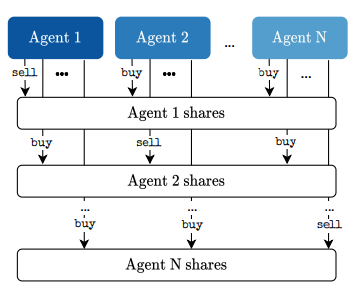
\includegraphics[width=0.48\linewidth]{pictures/SMG_sm.png}}
    \hspace{0.01\textwidth}
    %%----start of second subfigure----
    \subfloat[Action market]{
        \label{fig:am} %% label for second subfigure
        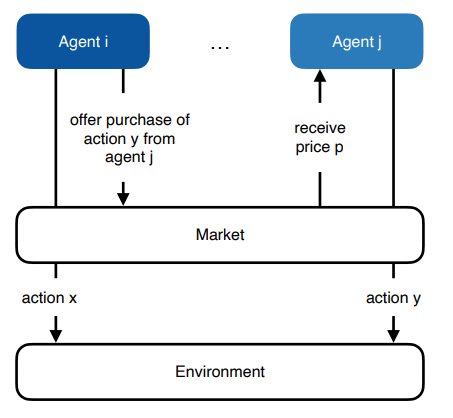
\includegraphics[width=0.41\linewidth]{pictures/SMG_am.png}}
    \caption[Illustrated Markets]{Illustrated Markets as defined in ``Stochastic Market Games'' \cite{scbe21} during one time step}
    \label{fig:multipic} %% label for entire figure
\end{figure}

If the buying offer coincide with a share that is up for sale in the same step, a market transaction is registered. Now, the shareholder participates in the reward of the current step of the transaction agent by a fixed dividend $d$. Schmid et al. mention that an optional price $p$ can be defined as an amount a seller receives from the buyer upon each share purchase. However, they claim that agents with high rewards are very likely to gift their shares in order to align the goals of the other agents with their own. Shareholders profit from the success of the selling party through the dividends.

% ------ ist das beispiel ok oder soll das raus? \\
An example here would be agent $i$ who wants to sell a share and agent $j$ that wants to buy a share specifically from agent $i$ with both being in time step $t$. In this scenario, the offers coincide and a share of $i$ is now claimed by $j$. If $i$ now receives a reward of one and the dividend is 20\%, agent $j$ would get a reward of 0.2 in addition to its own reward. However, in a scenario where agent $i$ decided not to sell, agent $j$ would not be able to claim the share and would not profit from the reward of agent $i$. After each step, the shares are resolved and the matching starts again.

On the contrary, the authors define conditional markets similar to purchase contracts, where buyers pay a fixed price $p$ to sellers when they in turn meet the buyers' demand. A proposed conditional SMG is the so-called action market (AM). In this case, actions are extended with a buying offer, containing one expected action from one specific agent, see figure \ref{fig:am}.

Again, in an example with two agents, $i$ and $j$, $i$ could need a resource that is currently occupied by $j$. Hence, agent $i$ would profit from $j$ giving up the resource and therefore offers to buy from $j$ the action ``release''. Formally, agent $i$ executes action $\overrightarrow{a}_{i,t}$ here, containing an environment action $a^{\text{env}}_{i,t}$ and the offer to agent $j$ $a^{\text{offer}}_{i,j,t}$ \cite{scbe21}. The offer proposal shows that agent $i$ is willing to buy from $j$ at time step $t$ a specific action $a^{\text{env}}_{j,t}$. If agent $j$ fulfills the conditions and releases the resource in the same step $t$, it would receive a fixed price from agent $i$ in form of reward. However, if that is not the case, the market conditions do not apply and $j$ is not paid by agent $i$.

In both market settings, a purchase is established if the specified agent happens to execute an action that matches with a buyer. It is important to emphasize, that the matching is performed during a time step, leaving it to chance, whether purchases take place. For instance, in an AM, agents do not know in advance if and what action another agent could be buying from them. Despite this uncertainty, the researchers showed, that both market implementations yielded promising results. An increase of the overall rewards of participating agents in mixed-motive games was seen.

%Vielleicht noch das Prisoner dilemma beispiel zeigen und in dem zug auch nash equi. erklären